\documentclass{report}
\iffalse
% gerby+plastex
\usepackage{amssymb, amsmath, hyperref}
\usepackage[backref]{natbib}
\else
% pure plastex / pdflatex
\usepackage{amssymb, amsmath, amsthm, hyperref}
\usepackage{natbib}
\fi
\newif\ifplastex
\plastexfalse
\ifplastex\else
\usepackage{cleveref}
\fi
\usepackage{tikz}
\usepackage{tikz-cd}

\theoremstyle{plain}
\newtheorem{theorem}[subsection]{Theorem}
\newtheorem{proposition}[subsection]{Proposition}
\newtheorem{lemma}[subsection]{Lemma}

\theoremstyle{definition}
\newtheorem{definition}[subsection]{Definition}
\newtheorem{example}[subsection]{Example}
\newtheorem{exercise}[subsection]{Exercise}
\newtheorem{situation}[subsection]{Situation}

\theoremstyle{remark}
\newtheorem{remark}[subsection]{Remark}
\newtheorem{remarks}[subsection]{Remarks}

\numberwithin{equation}{subsection}

\begin{document}

\chapter{A first chapter}
\label{chapter:first}

\section{A first section}

We can draw pictures using the \texttt{tikz} package.
\begin{center}
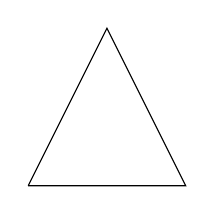
\begin{tikzpicture}
  \draw (0,0) --(1,2) -- (2,0) -- (0,0);
\end{tikzpicture}
\end{center}

We can also use the \texttt{tikz-cd} package for drawing commutative diagrams.
\begin{center}
\begin{tikzcd}
  a \arrow[r] & b
\end{tikzcd}
\end{center}

\label{section:first}

\begin{lemma}[Pythagorean theorem]
  \label{lemma:pythagoras}
  Let $a$, $b$, and $c$ be the sides of a right triangle, with $c$ being the hypotenuse. Then $a^2=b^2+c^2$ \cite{Euclid}.
\end{lemma}
\begin{proof}
  This is a consequence of the axioms of Euclidean geometry. It is left as an 
  exercise to the reader to verify that the proof of this lemma is correct. Or, see \cite{Euclid2} for a detailed proof.
\end{proof}




\section{A second section}
\label{section:second}


\chapter{A second chapter}
\label{chapter:second}

\begin{definition}[Pythagorean triple]
  \label{definition:pythagorean-triple}
  A triple of positive integers $(a,b,c)$ is called a \emph{Pythagorean triple} if $a^2=b^2+c^2$.
\end{definition}

\begin{theorem}[Pythagorean triples]
  \label{theorem:pythagorean-triple}
  There are infinitely many Pythagorean triples.
\end{theorem}
\begin{proof}
  For each positive integer $n$, we have the triple $(a,b,c)=(n^2+1, n^2-1, 2n)$, which satisfies $a^2=b^2+c^2$. Indeed, we have
  \begin{align*}
    a^2 &= (n^2+1)^2 = n^4 + 2n^2 + 1, \\
    b^2 &= (n^2-1)^2 = n^4 - 2n^2 + 1, \\ 
    c^2 &= (2n)^2 = 4n^2.
  \end{align*}
  Therefore,
  \begin{align*}
    a^2 - b^2 &= (n^4 + 2n^2 + 1) - (n^4 - 2n^2 + 1) = 4n^2 = c^2.
  \end{align*}
\end{proof}

\begin{example}
  \label{example:pythagorean-triple}
  The triple $(3,4,5)$ is a Pythagorean triple, since $3^2=4^2+5^2$. This example is a special case of the construction given in the proof of \Cref{theorem:pythagorean-triple}, since it corresponds to the case $n=2$.
\end{example}

\section{A third section}
\label{section:third}


\section{A fourth section}
\label{section:fourth}

\bibliographystyle{plainnat}
\bibliography{references}

\end{document}
